% Options for packages loaded elsewhere
% Options for packages loaded elsewhere
\PassOptionsToPackage{unicode}{hyperref}
\PassOptionsToPackage{hyphens}{url}
\PassOptionsToPackage{dvipsnames,svgnames,x11names}{xcolor}
%
\documentclass[
  letterpaper,
  DIV=11,
  numbers=noendperiod]{scrartcl}
\usepackage{xcolor}
\usepackage{amsmath,amssymb}
\setcounter{secnumdepth}{-\maxdimen} % remove section numbering
\usepackage{iftex}
\ifPDFTeX
  \usepackage[T1]{fontenc}
  \usepackage[utf8]{inputenc}
  \usepackage{textcomp} % provide euro and other symbols
\else % if luatex or xetex
  \usepackage{unicode-math} % this also loads fontspec
  \defaultfontfeatures{Scale=MatchLowercase}
  \defaultfontfeatures[\rmfamily]{Ligatures=TeX,Scale=1}
\fi
\usepackage{lmodern}
\ifPDFTeX\else
  % xetex/luatex font selection
\fi
% Use upquote if available, for straight quotes in verbatim environments
\IfFileExists{upquote.sty}{\usepackage{upquote}}{}
\IfFileExists{microtype.sty}{% use microtype if available
  \usepackage[]{microtype}
  \UseMicrotypeSet[protrusion]{basicmath} % disable protrusion for tt fonts
}{}
\makeatletter
\@ifundefined{KOMAClassName}{% if non-KOMA class
  \IfFileExists{parskip.sty}{%
    \usepackage{parskip}
  }{% else
    \setlength{\parindent}{0pt}
    \setlength{\parskip}{6pt plus 2pt minus 1pt}}
}{% if KOMA class
  \KOMAoptions{parskip=half}}
\makeatother
% Make \paragraph and \subparagraph free-standing
\makeatletter
\ifx\paragraph\undefined\else
  \let\oldparagraph\paragraph
  \renewcommand{\paragraph}{
    \@ifstar
      \xxxParagraphStar
      \xxxParagraphNoStar
  }
  \newcommand{\xxxParagraphStar}[1]{\oldparagraph*{#1}\mbox{}}
  \newcommand{\xxxParagraphNoStar}[1]{\oldparagraph{#1}\mbox{}}
\fi
\ifx\subparagraph\undefined\else
  \let\oldsubparagraph\subparagraph
  \renewcommand{\subparagraph}{
    \@ifstar
      \xxxSubParagraphStar
      \xxxSubParagraphNoStar
  }
  \newcommand{\xxxSubParagraphStar}[1]{\oldsubparagraph*{#1}\mbox{}}
  \newcommand{\xxxSubParagraphNoStar}[1]{\oldsubparagraph{#1}\mbox{}}
\fi
\makeatother

\usepackage{color}
\usepackage{fancyvrb}
\newcommand{\VerbBar}{|}
\newcommand{\VERB}{\Verb[commandchars=\\\{\}]}
\DefineVerbatimEnvironment{Highlighting}{Verbatim}{commandchars=\\\{\}}
% Add ',fontsize=\small' for more characters per line
\usepackage{framed}
\definecolor{shadecolor}{RGB}{241,243,245}
\newenvironment{Shaded}{\begin{snugshade}}{\end{snugshade}}
\newcommand{\AlertTok}[1]{\textcolor[rgb]{0.68,0.00,0.00}{#1}}
\newcommand{\AnnotationTok}[1]{\textcolor[rgb]{0.37,0.37,0.37}{#1}}
\newcommand{\AttributeTok}[1]{\textcolor[rgb]{0.40,0.45,0.13}{#1}}
\newcommand{\BaseNTok}[1]{\textcolor[rgb]{0.68,0.00,0.00}{#1}}
\newcommand{\BuiltInTok}[1]{\textcolor[rgb]{0.00,0.23,0.31}{#1}}
\newcommand{\CharTok}[1]{\textcolor[rgb]{0.13,0.47,0.30}{#1}}
\newcommand{\CommentTok}[1]{\textcolor[rgb]{0.37,0.37,0.37}{#1}}
\newcommand{\CommentVarTok}[1]{\textcolor[rgb]{0.37,0.37,0.37}{\textit{#1}}}
\newcommand{\ConstantTok}[1]{\textcolor[rgb]{0.56,0.35,0.01}{#1}}
\newcommand{\ControlFlowTok}[1]{\textcolor[rgb]{0.00,0.23,0.31}{\textbf{#1}}}
\newcommand{\DataTypeTok}[1]{\textcolor[rgb]{0.68,0.00,0.00}{#1}}
\newcommand{\DecValTok}[1]{\textcolor[rgb]{0.68,0.00,0.00}{#1}}
\newcommand{\DocumentationTok}[1]{\textcolor[rgb]{0.37,0.37,0.37}{\textit{#1}}}
\newcommand{\ErrorTok}[1]{\textcolor[rgb]{0.68,0.00,0.00}{#1}}
\newcommand{\ExtensionTok}[1]{\textcolor[rgb]{0.00,0.23,0.31}{#1}}
\newcommand{\FloatTok}[1]{\textcolor[rgb]{0.68,0.00,0.00}{#1}}
\newcommand{\FunctionTok}[1]{\textcolor[rgb]{0.28,0.35,0.67}{#1}}
\newcommand{\ImportTok}[1]{\textcolor[rgb]{0.00,0.46,0.62}{#1}}
\newcommand{\InformationTok}[1]{\textcolor[rgb]{0.37,0.37,0.37}{#1}}
\newcommand{\KeywordTok}[1]{\textcolor[rgb]{0.00,0.23,0.31}{\textbf{#1}}}
\newcommand{\NormalTok}[1]{\textcolor[rgb]{0.00,0.23,0.31}{#1}}
\newcommand{\OperatorTok}[1]{\textcolor[rgb]{0.37,0.37,0.37}{#1}}
\newcommand{\OtherTok}[1]{\textcolor[rgb]{0.00,0.23,0.31}{#1}}
\newcommand{\PreprocessorTok}[1]{\textcolor[rgb]{0.68,0.00,0.00}{#1}}
\newcommand{\RegionMarkerTok}[1]{\textcolor[rgb]{0.00,0.23,0.31}{#1}}
\newcommand{\SpecialCharTok}[1]{\textcolor[rgb]{0.37,0.37,0.37}{#1}}
\newcommand{\SpecialStringTok}[1]{\textcolor[rgb]{0.13,0.47,0.30}{#1}}
\newcommand{\StringTok}[1]{\textcolor[rgb]{0.13,0.47,0.30}{#1}}
\newcommand{\VariableTok}[1]{\textcolor[rgb]{0.07,0.07,0.07}{#1}}
\newcommand{\VerbatimStringTok}[1]{\textcolor[rgb]{0.13,0.47,0.30}{#1}}
\newcommand{\WarningTok}[1]{\textcolor[rgb]{0.37,0.37,0.37}{\textit{#1}}}

\usepackage{longtable,booktabs,array}
\usepackage{calc} % for calculating minipage widths
% Correct order of tables after \paragraph or \subparagraph
\usepackage{etoolbox}
\makeatletter
\patchcmd\longtable{\par}{\if@noskipsec\mbox{}\fi\par}{}{}
\makeatother
% Allow footnotes in longtable head/foot
\IfFileExists{footnotehyper.sty}{\usepackage{footnotehyper}}{\usepackage{footnote}}
\makesavenoteenv{longtable}
\usepackage{graphicx}
\makeatletter
\newsavebox\pandoc@box
\newcommand*\pandocbounded[1]{% scales image to fit in text height/width
  \sbox\pandoc@box{#1}%
  \Gscale@div\@tempa{\textheight}{\dimexpr\ht\pandoc@box+\dp\pandoc@box\relax}%
  \Gscale@div\@tempb{\linewidth}{\wd\pandoc@box}%
  \ifdim\@tempb\p@<\@tempa\p@\let\@tempa\@tempb\fi% select the smaller of both
  \ifdim\@tempa\p@<\p@\scalebox{\@tempa}{\usebox\pandoc@box}%
  \else\usebox{\pandoc@box}%
  \fi%
}
% Set default figure placement to htbp
\def\fps@figure{htbp}
\makeatother





\setlength{\emergencystretch}{3em} % prevent overfull lines

\providecommand{\tightlist}{%
  \setlength{\itemsep}{0pt}\setlength{\parskip}{0pt}}



 


\KOMAoption{captions}{tableheading}
\makeatletter
\@ifpackageloaded{caption}{}{\usepackage{caption}}
\AtBeginDocument{%
\ifdefined\contentsname
  \renewcommand*\contentsname{Table of contents}
\else
  \newcommand\contentsname{Table of contents}
\fi
\ifdefined\listfigurename
  \renewcommand*\listfigurename{List of Figures}
\else
  \newcommand\listfigurename{List of Figures}
\fi
\ifdefined\listtablename
  \renewcommand*\listtablename{List of Tables}
\else
  \newcommand\listtablename{List of Tables}
\fi
\ifdefined\figurename
  \renewcommand*\figurename{Figure}
\else
  \newcommand\figurename{Figure}
\fi
\ifdefined\tablename
  \renewcommand*\tablename{Table}
\else
  \newcommand\tablename{Table}
\fi
}
\@ifpackageloaded{float}{}{\usepackage{float}}
\floatstyle{ruled}
\@ifundefined{c@chapter}{\newfloat{codelisting}{h}{lop}}{\newfloat{codelisting}{h}{lop}[chapter]}
\floatname{codelisting}{Listing}
\newcommand*\listoflistings{\listof{codelisting}{List of Listings}}
\makeatother
\makeatletter
\makeatother
\makeatletter
\@ifpackageloaded{caption}{}{\usepackage{caption}}
\@ifpackageloaded{subcaption}{}{\usepackage{subcaption}}
\makeatother
\usepackage{bookmark}
\IfFileExists{xurl.sty}{\usepackage{xurl}}{} % add URL line breaks if available
\urlstyle{same}
\hypersetup{
  pdftitle={mini\_case\_report},
  colorlinks=true,
  linkcolor={blue},
  filecolor={Maroon},
  citecolor={Blue},
  urlcolor={Blue},
  pdfcreator={LaTeX via pandoc}}


\title{mini\_case\_report}
\author{}
\date{}
\begin{document}
\maketitle


\begin{Shaded}
\begin{Highlighting}[]
\FunctionTok{library}\NormalTok{(tidyverse)}
\end{Highlighting}
\end{Shaded}

\begin{verbatim}
-- Attaching core tidyverse packages ------------------------ tidyverse 2.0.0 --
v dplyr     1.2.0     v readr     2.2.0
v forcats   1.0.1     v stringr   1.6.0
v ggplot2   4.0.2     v tibble    3.3.1
v lubridate 1.9.5     v tidyr     1.3.2
v purrr     1.2.1     
-- Conflicts ------------------------------------------ tidyverse_conflicts() --
x dplyr::filter() masks stats::filter()
x dplyr::lag()    masks stats::lag()
i Use the conflicted package (<http://conflicted.r-lib.org/>) to force all conflicts to become errors
\end{verbatim}

\begin{Shaded}
\begin{Highlighting}[]
\NormalTok{gym\_raw }\OtherTok{\textless{}{-}} \FunctionTok{read\_csv}\NormalTok{(}\StringTok{"../data/gym\_membership\_behavior.csv"}\NormalTok{)}
\end{Highlighting}
\end{Shaded}

\begin{verbatim}
Rows: 260 Columns: 11
-- Column specification --------------------------------------------------------
Delimiter: ","
chr (3): membership_type, branch_region, cancelled_last_60d
dbl (8): member_id, months_as_member, visits_last_30d, avg_visit_minutes, pe...

i Use `spec()` to retrieve the full column specification for this data.
i Specify the column types or set `show_col_types = FALSE` to quiet this message.
\end{verbatim}

\begin{Shaded}
\begin{Highlighting}[]
\FunctionTok{source}\NormalTok{(}\StringTok{"../scripts/02\_prepare\_data.R"}\NormalTok{)}
\end{Highlighting}
\end{Shaded}

\begin{verbatim}
Rows: 260
Columns: 11
$ member_id                  <dbl> 5001, 5002, 5003, 5004, 5005, 5006, 5007, 5~
$ membership_type            <chr> "Premium", "Standard", "Premium", "Basic", ~
$ branch_region              <chr> "Öst", "Öst", "Öst", "Väst", "Nord", "Öst",~
$ months_as_member           <dbl> 22, 3, 16, 1, 31, 6, 1, 28, 21, 30, 21, 11,~
$ visits_last_30d            <dbl> 11, 6, 7, 3, 11, 3, 2, 4, 8, 8, 10, 5, 7, 1~
$ avg_visit_minutes          <dbl> 67.6, 59.0, 46.6, 57.5, 84.3, 70.0, 71.7, 4~
$ personal_training_sessions <dbl> 0, 0, 1, 0, 0, 1, 2, 0, 0, 0, 0, 0, 0, 1, 1~
$ app_engagement_score       <dbl> 79.1, 64.3, 65.4, 31.7, 99.9, 35.8, 47.2, 8~
$ monthly_spend              <dbl> 897.92, 473.09, 993.02, 335.31, 410.18, 663~
$ cancelled_last_60d         <chr> "No", "No", "No", "No", "No", "Yes", "No", ~
$ satisfaction_score         <dbl> 9.1, 7.9, 9.9, 7.3, NA, 6.5, 9.1, 5.6, 8.4,~
Rows: 260
Columns: 13
$ member_id                  <dbl> 5001, 5002, 5003, 5004, 5005, 5006, 5007, 5~
$ membership_type            <fct> Premium, Standard, Premium, Basic, Basic, S~
$ branch_region              <fct> Öst, Öst, Öst, Väst, Nord, Öst, Väst, Nord,~
$ months_as_member           <dbl> 22, 3, 16, 1, 31, 6, 1, 28, 21, 30, 21, 11,~
$ visits_last_30d            <dbl> 11, 6, 7, 3, 11, 3, 2, 4, 8, 8, 10, 5, 7, 1~
$ avg_visit_minutes          <dbl> 67.6, 59.0, 46.6, 57.5, 84.3, 70.0, 71.7, 4~
$ personal_training_sessions <dbl> 0, 0, 1, 0, 0, 1, 2, 0, 0, 0, 0, 0, 0, 1, 1~
$ app_engagement_score       <dbl> 79.1, 64.3, 65.4, 31.7, 99.9, 35.8, 47.2, 8~
$ monthly_spend              <dbl> 897.92, 473.09, 993.02, 335.31, 410.18, 663~
$ cancelled_last_60d         <fct> No, No, No, No, No, Yes, No, No, No, No, No~
$ satisfaction_score         <dbl> 9.1, 7.9, 9.9, 7.3, NA, 6.5, 9.1, 5.6, 8.4,~
$ high_engagement            <fct> High, Lower, Lower, Lower, High, Lower, Low~
$ spend_per_visit            <dbl> 81.62909, 78.84833, 141.86000, 111.77000, 3~
\end{verbatim}

\begin{Shaded}
\begin{Highlighting}[]
\FunctionTok{source}\NormalTok{(}\StringTok{"../scripts/03\_analysis.R"}\NormalTok{)}
\FunctionTok{source}\NormalTok{(}\StringTok{"../scripts/04\_figures.R"}\NormalTok{)}
\end{Highlighting}
\end{Shaded}

\section{Introduktion}\label{introduktion}

I den här rapporten analyseras medlemsbeteende i en träningskedja. Fokus
ligger på två frågor: hur medlemskapstyperna skiljer sig åt i användning
och spend, och om det finns tecken på att lägre engagemang hänger ihop
med avhopp.

\section{Fråga 1}\label{fruxe5ga-1}

Hur skiljer sig medlemskapstyperna åt i användning och spend?

\begin{Shaded}
\begin{Highlighting}[]
\NormalTok{membership\_summary}
\end{Highlighting}
\end{Shaded}

\begin{verbatim}
# A tibble: 3 x 8
  membership_type avg_visits median_visits avg_spend median_spend avg_minutes
  <fct>                <dbl>         <dbl>     <dbl>        <dbl>       <dbl>
1 Basic                 5.96             5      396.         386.        52.9
2 Premium               8.05             7     1100.        1059.        66.9
3 Standard              6.89             7      644.         591.        57.7
# i 2 more variables: avg_pt <dbl>, n <int>
\end{verbatim}

\begin{Shaded}
\begin{Highlighting}[]
\NormalTok{p\_spend\_membership}
\end{Highlighting}
\end{Shaded}

\begin{verbatim}
Warning: Removed 7 rows containing non-finite outside the scale range
(`stat_boxplot()`).
\end{verbatim}

\pandocbounded{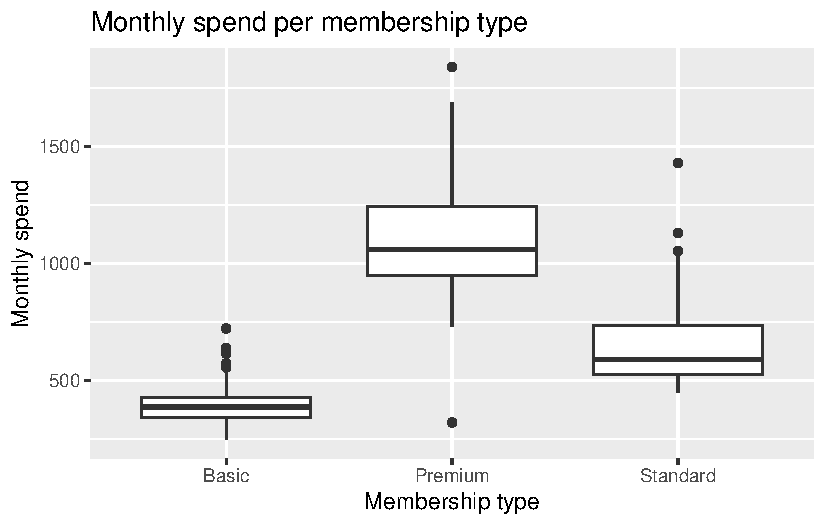
\includegraphics[keepaspectratio]{mini_case_report_files/figure-pdf/unnamed-chunk-3-1.pdf}}

Premium-medlemmar verkar ha tydligt högre monthly spend än både Standard
och Basic. Standard ligger i mitten, medan Basic ligger lägst. Figuren
visar också att spridningen är större i Premium-gruppen än i
Basic-gruppen.

\begin{Shaded}
\begin{Highlighting}[]
\NormalTok{p\_visits\_membership}
\end{Highlighting}
\end{Shaded}

\pandocbounded{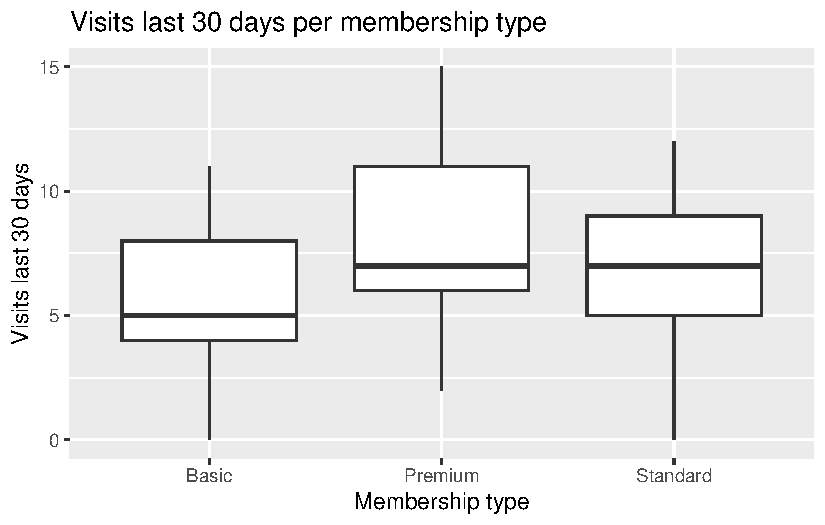
\includegraphics[keepaspectratio]{mini_case_report_files/figure-pdf/unnamed-chunk-4-1.pdf}}

Antal besök verkar också skilja sig mellan grupperna. Premium ligger
högst även här, medan Basic ligger lägre. Skillnaderna är tydliga, även
om de inte är lika stora som för spend.

\section{Fråga 2}\label{fruxe5ga-2}

Finns det tecken på att lägre engagemang hänger ihop med avhopp?

\begin{Shaded}
\begin{Highlighting}[]
\NormalTok{cancellation\_summary}
\end{Highlighting}
\end{Shaded}

\begin{verbatim}
# A tibble: 2 x 8
  cancelled_last_60d avg_visits median_visits avg_app median_app
  <fct>                   <dbl>         <dbl>   <dbl>      <dbl>
1 No                       7.08           7      67.2       67.1
2 Yes                      5.52           5.5    60.7       58.9
# i 3 more variables: avg_satisfaction <dbl>, median_satisfaction <dbl>,
#   n <int>
\end{verbatim}

\begin{Shaded}
\begin{Highlighting}[]
\NormalTok{p\_satisfaction\_cancel}
\end{Highlighting}
\end{Shaded}

\begin{verbatim}
Warning: Removed 5 rows containing non-finite outside the scale range
(`stat_boxplot()`).
\end{verbatim}

\pandocbounded{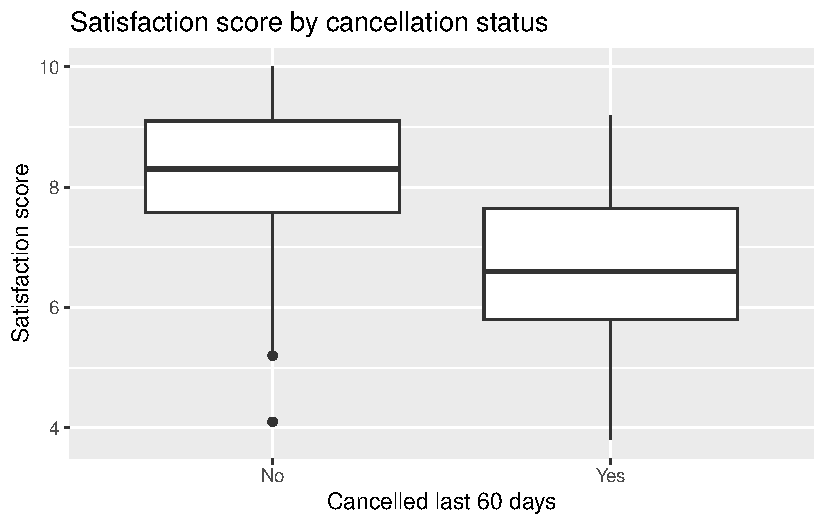
\includegraphics[keepaspectratio]{mini_case_report_files/figure-pdf/unnamed-chunk-6-1.pdf}}

\begin{Shaded}
\begin{Highlighting}[]
\NormalTok{cancel\_test}
\end{Highlighting}
\end{Shaded}

\begin{verbatim}

    Welch Two Sample t-test

data:  app_engagement_score by cancelled_last_60d
t = 2.7565, df = 59.774, p-value = 0.007736
alternative hypothesis: true difference in means between group No and group Yes is not equal to 0
95 percent confidence interval:
  1.800125 11.326693
sample estimates:
 mean in group No mean in group Yes 
         67.24591          60.68250 
\end{verbatim}




\end{document}
